% Lexsi Stage 2 short paper. Build: latexmk -pdf paper.tex (in this folder).
\documentclass[11pt]{article}
\usepackage[final]{acl}
\usepackage{times}
\usepackage{latexsym}
\usepackage[T1]{fontenc}
\usepackage[utf8]{inputenc}
\usepackage{microtype}
\usepackage{inconsolata}
\usepackage{graphicx}
\usepackage{booktabs}
\usepackage{amsmath}
\usepackage{amssymb}
\usepackage{xcolor}
\graphicspath{{../figures/}}
\newcommand{\pending}[1]{\textcolor{red}{[#1]}}

\title{Weights and Harness Are Complements: Distilling a Scientific Strategy Investigator into an 8B Model}

\author{Hatem Saadallah \and Nour Jennane}

\begin{document}
\maketitle

\begin{abstract}
Asked whether a manufacturer should take its technology to a new kind of customer, language models write consulting
prose; good strategy work instead frames the decision, states rival causal theories, weighs evidence for and against
each, designs a test that separates them, and revises on new evidence. We distil that procedure from a Command~A+
teacher into Aya Expanse 8B, trained with AgentTune and Unsloth inside an executable environment of twelve guarded
tools, and measure what each part of the agent contributes. On development cases (one blind judge, 45 paired runs per
arm), fine-tuning on an identical scaffold lifts the 8B from finishing 9\% of investigations to 87\% and raises judged
quality by +0.72, +0.88 and +0.77 on a 0 to 3 rubric at three training seeds, every interval above zero, with general
ability unchanged (+0.6 points on MMLU and ARC). The trained weights do not replace the harness around them: on the
held-out test, removing the decoding guards costs $-0.48$ [$-0.65$, $-0.31$] at all twelve companies (finished runs
81 to 34), and on development serving the base model for the late stages costs $-0.19$. Data changes matter less than expected or backfire: correction rows move a checkable error but not quality,
rule-built recovery rows and teacher corrections of the student's own failure states each gained at one training seed and vanished over three (pooled +0.02 and $-0.03$), so
single-seed gains in agent fine-tuning should not be trusted, and rebalancing the teacher's data toward rare skills makes the agent fragile, collapsing into loops at two of three
training seeds ($-0.72$ [$-0.92$, $-0.50$] pooled). A decision model for one typed
choice improves labels, not judged quality. On a fresh test set of twelve companies, run once and read by two judges,
the fine-tuned 8B beats the same model prompted on the same scaffold by \textbf{+0.70 [0.61, 0.79]} (interval over
companies), at all twelve companies, and finishes 81 of 96 investigations against 2.
\end{abstract}

\section{Introduction}

The Lexsi AI Hackathon ran in two stages. In Stage~1 we built aemon, an environment of guarded tools for a
scientific investigation of a strategy question \citep{camuffo2020scientific,camuffo2024theory}, and showed that a
small open model (Tiny Aya 3.35B) learns its form by copying a teacher's tool calls, beating its prompted base on two
frozen tests. This paper is Stage~2. Stage~1 also showed where the student stops: it learns the procedure better than the
judgement, and fails mechanically by looping and by citing simulated results. The agent is the model plus the steps
around it: its training data, the decoding constraints on each call, and the choices it makes itself.

\begin{figure}[t]
\centering
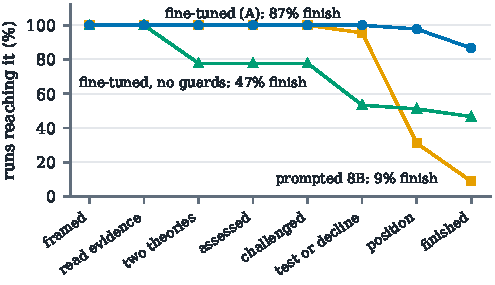
\includegraphics[width=\columnwidth]{fig_stages.pdf}
\caption{How far each agent gets: the share of all 45 development runs (15 cases, 3 attempts) that complete each
stage, with the same scaffold, decoding guards and server. Prompted, Aya Expanse 8B stops before stating a position in
most runs (repeated errors); fine-tuned (A) it finishes 87\%; without the guards the fine-tuned agent loses a fifth of
its runs at the theories stage. Blind judged quality: 1.29, 2.01 and 1.57 of 3.}
\label{fig:stages}
\end{figure}

We make three contributions.
\begin{enumerate}
\item \textbf{Agent fine-tuning measured part by part.} An 8B Cohere student (Aya Expanse 8B) trained with AgentTune
on the Stage~1 teacher data, and ablations of the guards, the training data (correction rows, rule-built recovery
rows, a skill-balanced composition, teacher corrections of the student's own failure states) and the prompt, each against one
reference with matched training seeds (Sections~\ref{sec:method} and~\ref{sec:results}).
\item \textbf{Weights and harness are complements.} Fine-tuning moves the 8B from finishing 9\% of runs to 87\%
on an identical scaffold (Figure~\ref{fig:stages}), yet the fine-tuned agent still needs its decoding guards, needs its
adapter in the late stages, and breaks when its data are naively rebalanced; general ability is unchanged, and a
decision model for one typed choice improves labels but not judged quality (Section~\ref{sec:results}).
\item \textbf{An honest test.} A fresh test set of twelve companies chosen by a committed rule, 230 records verified
against their live pages, four cases per company including supporting and contradicting simulated evidence, frozen
before any result of the fine-tuned 8B was opened; two blind judges; company-level intervals (Section~\ref{sec:test3}).
\end{enumerate}

\section{Task, environment and tests}

\subsection{Task and environment (from Stage~1)}

A case fixes a company, a question (``Should X develop a differentiated consumer proposition for a specific use case,
beyond its existing offer? What evidence would justify that investment?''), a brief, budgets and a dossier of
verified public records. The agent acts only through twelve guarded tools: frame the problem; search and read
sources; add theories with an explicit causal mechanism; assess a quoted passage against a theory, with its direction,
its kind and what it does not show; challenge the favoured theory; propose a test with predictions per theory and a
decision rule, or decline one; state a position with a belief per theory; revise after new evidence; finish. A stage
controller opens only the current step's tools. Guards refuse what the procedure forbids: a quote that is not in the
source, a theory that repeats another, a simulated result cited as support or in the recommendation. Every run is
recorded and replayed with AuditKIT \citep{lexsi_auditkit}, which re-executes every recorded tool call through the
guarded tools and scores the calls; eleven development audits skipped at run time were run afterwards on the saved
trajectories (Section~\ref{sec:analysis}).

\subsection{Development and the earlier tests}

Development uses 15 cases of six validation companies, 3 attempts each (45 runs per arm), and one qualified blind
judge (codexsol170: the Codex CLI on gpt-6-sol). The \emph{Stage~1 system} is Tiny Aya Global 3.35B with two
adapters (one gathers the evidence, one trained on a second teacher's runs reasons) and the same six guards. Stage~1's two test sets have been read, so we use neither as a test.

\subsection{Test set 3}
\label{sec:test3}

Twelve companies: five chosen first (Eberspächer, Gühring, Krones, Lapp, MULTIVAC) and seven drawn by a written rule
committed before any dossier research began (Kardex, Nabtesco, Biesse, Brembo, Rieter, Sika, Tomra): manufacturers mainly
selling to businesses, EUR 0.3 to 15 billion in revenue, absent from every case file and proposal, outside every
development and test company's product category, covering twelve sectors and five countries. Records are short
verbatim excerpts from public pages, checked mechanically against the live page; of 262 gathered, 230 were verified
and admitted and the rest dropped unedited. Each company has four cases: base, irrelevant simulated evidence, and a
pair of simulated randomized offer tests on one narrow mechanism (for example installation friction for parking
heaters) whose two versions share the record's id and title and differ only in mirrored outcome counts (72 against 32
of 400 per arm). The tools refuse that record as support for a theory or as cited evidence. Leakage and searchability
checks pass, and the set was frozen before any result of the fine-tuned 8B was opened (commit \texttt{f5e0b6b} in our private repository, readable on request, 19 November; content
sha256 \texttt{068261a91fb3d8b8\ldots}): 48 cases $\times$ 2 attempts = 96 runs per arm. Against the 1,554 records of
the training and development dossiers, the closest test record has a character n-gram TF-IDF cosine of 0.44 (median
nearest neighbour 0.17); the closest pairs are generic company-size sentences, not shared content.

\section{Method}
\label{sec:method}

\subsection{Student and training}

The student is Aya Expanse 8B (CohereLabs, revision \texttt{5062468b}, CC-BY-NC-4.0); the trained agent stays a Cohere
model, as the track requires. The data are 3,891 replay-exact Command~A+ tool-call rows from 158 investigations on 57
training companies plus 51 correction rows (3,942 in all), about 410,000 supervised tokens, with the loss on the target call only.
LoRA \citep{hu2022lora} has rank 16, alpha 32 and dropout 0.05 on all seven linear projections of each block (224
modules, 41.9M trainable parameters); training runs two epochs, 1,971 optimizer steps, at learning rate $10^{-4}$,
through AgentTune's distillation trainer \citep{lexsi_agenttune,hinton2015distilling}, with Unsloth building the model
and adapters. Each row $r$ pairs the context $x_r$ the student saw with the teacher's next call $y_r$, and only the call's
tokens carry loss:
\begin{equation}
\mathcal{L}(\theta) = -\frac{1}{\sum_r |y_r|} \sum_r \sum_{t=1}^{|y_r|} \log p_\theta\!\left(y_{r,t} \mid x_r, y_{r,<t}\right),
\end{equation}
with extra rows $E$ (corrections, recovery rows) capped at $\sum_{r \in E} |y_r| \le 0.2 \sum_r |y_r|$. Each adapted
weight is $W' = W + \tfrac{\alpha}{k} BA$ with $B \in \mathbb{R}^{d \times k}$, $A \in \mathbb{R}^{k \times m}$, rank
$k = 16$ and $\alpha = 32$; only $A$ and $B$ train. Held-out loss on 240 rows of the six validation companies fell from 0.565 to 0.387. There is no
checkpoint selection: every adapter is the last step of the fixed schedule, and configurations are chosen on
development only, by the rule registered in Section~\ref{sec:test3run}.

\subsection{Serving and the checks that make a comparison fair}

Every arm serves a bf16 GGUF converted in the job from the pinned weights, so no third-party conversion or
quantization differs between arms. Before any run the job checks that the server's tokens for a training row's
context are identical to the tokens training used, and, with an adapter, that a request with the adapter off leaves
the next agent request's log-probabilities unchanged.

\subsection{The decision model}
\label{sec:decide-method}

One typed choice, the evidence kind of each third-party quote, can be taken from the agent and decided by the base
weights' option-letter log-probabilities, abstaining below a fixed confidence (Appendix~\ref{app:decide}).

\section{Results}
\label{sec:results}

All development numbers use one judge (codexsol170), 15 cases and 45 runs per arm. One judge suffices for
comparing arms because in Stage~1 our two judges (Claude and a Codex model) agreed on order but not on level: their run
scores rank-correlated 0.90 to 0.95 over five campaigns of 60 to 360 runs, they put all five arms of test set 2 in the
same order, and they differed only in level (Codex higher by 0.3 to 0.4 per run) and in the order of two arms
0.05 apart. We therefore compare arms with one judge on development, report differences rather than levels, and
add the second judge for the test. A run's score is the mean of its
judged dimensions, $s = \tfrac{1}{|D|}\sum_{d \in D} s_d$ with $s_d \in \{0,1,2,3\}$ and an unreached dimension
scored 0. Two arms are compared run by run, $\delta_{c,a} = s^{(1)}_{c,a} - s^{(2)}_{c,a}$ for case $c$ and attempt $a$,
and we report $\hat\Delta = \operatorname{mean}_{c,a} \delta_{c,a}$ with a 95\% percentile interval from 4,000 bootstrap
resamples of cases, each case keeping all its attempts. Test set 3 adds two judges and an interval over its 12
companies (Section~\ref{sec:test3run}).

\subsection{Does fine-tuning the 8B help?}

\begin{table}[t]
\centering
\small
\setlength{\tabcolsep}{2.5pt}
\begin{tabular}{lcccc}
\toprule
Development & Score & Fin. & No-test & vs St.\,1 \\
\midrule
Stage 1 system (3.35B) & 1.88 & 43 & 6/6 & -- \\
8B prompted, staged & 1.41 & 27 & & $-0.47$ \\
8B prompted, same & 1.29 & 4 & 4/6 & $-0.59$ \\
A: 8B fine-tuned & 2.01 & 39 & 6/6 & $+0.13$ \\
B: A + recovery & 2.19 & 45 & 6/6 & $+0.31$ \\
A, seed 11 & 2.17 & 41 & 6/6 & $+0.29$ \\
B, seed 11 & 1.97 & 41 & 6/6 & $+0.09$ \\
A, seed 13 & 2.06 & 39 & 6/6 & $+0.18$ \\
B, seed 13 & 2.14 & 42 & 6/6 & $+0.26$ \\
\bottomrule
\end{tabular}
\caption{Judge score (0 to 3) and runs finished of 45; rows without a seed are training seed 7. No-test: runs that propose a test on the two
cases labelled as not warranting one (6 runs; labels contestable). No arm ever declines a test or ends with
``insufficient evidence''. Intervals in the text.}
\label{tab:main}
\end{table}

\begin{figure}[t]
\centering
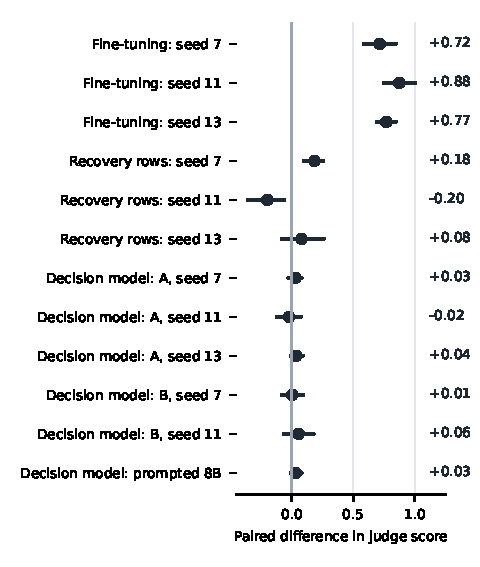
\includegraphics[width=\columnwidth]{fig_seeds.pdf}
\caption{Paired effects on development at each training seed (one judge, 45 runs per arm): mean difference with its
95\% interval. Fine-tuning is A against the prompted 8B on the same scaffold; recovery rows are B minus A at the same
seed; the decision model is on minus off.}
\label{fig:effects}
\end{figure}

\paragraph{Fine-tuning, isolated.} Against the same 8B prompted with the identical prompt, guards, context and
precision, the fine-tuned agent scores +0.72 [+0.59, +0.85] higher at training seed 7, at all six companies, and finishes 39 runs
against 4 (Table~\ref{tab:main}, Figure~\ref{fig:effects}). The prompted model mostly fails at the procedure itself:
140 of its 265 refused calls state a position before challenging the favoured theory. The gap is largest on the
recommendation (1.16 against 0.09) and revision (2.33 against 0.30). Against the prompted 8B under its best prompt
(staged), the gain is +0.60 [+0.49, +0.70]. The gain is not only finishing: compared only on the rubric dimensions
both runs reached (7.2 of 9 on average), as in Stage~1, A leads by +0.59 [+0.45, +0.72], +0.73 [+0.61, +0.85] and
+0.62 [+0.54, +0.68] at seeds 7, 11 and 13; finishing more of the procedure accounts for 0.13 to 0.15 of it.

\paragraph{Two model sizes.} The same comparison, fine-tuned against prompted base, gave +0.83 [0.69, 0.97] for Tiny
Aya Global (3.35B) on Stage~1's frozen final test with two judges, and gives +0.72 to +0.88 for Aya Expanse 8B
on development with one judge. The splits, judges and scaffolds differ (a test result with two judges against a development
result with one), so only the direction and rough size agree; on test set 3, with two judges, the 8B
gain is +0.70 [0.61, 0.79] (Section~\ref{sec:test3run}).

Against the Stage~1 system the fine-tuned 8B is ahead by +0.13 [+0.03, +0.23], +0.29 [+0.18, +0.39] and +0.18
[+0.09, +0.27] at seeds 7, 11 and 13, with the largest gains on revision and distinct theories, but finishes 39, 41 and
39 runs against its 43; on test set 3 the gap is +0.12 [+0.05, +0.20].

\subsection{Which parts of the agent earn their place?}
\label{sec:parts}

\paragraph{Recovery rows.} Adding 401 rule-built recovery rows (the student's two common mistakes, a repeated call
and a simulated result cited in the recommendation, each followed by the teacher's own next call) removes the loops at
seed 7 (45 of 45 finished; refused calls 28 against 146) and gains +0.18 [+0.10, +0.25] over A. It does not replicate:
B minus A is $-0.20$ [$-0.36$, $-0.06$] at seed 11 (330 refused calls, loops at one company) and +0.08 [$-0.08$, +0.26]
at seed 13; pooled over seeds +0.02 [$-0.04$, +0.09], while B finishes 128 runs against 119. B fails its registered
admission rule, and A is the configuration for test set 3. B's data trained for A's 1,971 steps collapses to 0.65,
looping in the theories stage: the rows make the agent finish more often but loop unpredictably across training runs.

\paragraph{Correction rows.} Without A's 51 correction rows (seed 7) quality is unchanged (+0.01 [$-0.12$, +0.12]),
37 runs finish against 39, and the agent cites simulated results as evidence 32 times against 20 with them: a
checkable error the rows were written for moves, judged quality does not. Without them the agent is still +0.72
[+0.56, +0.87] above the prompted 8B.

\paragraph{Corrections of the student's own states.} One round of teacher corrections on 148 states where A failed
(40 kept by the checks) gains +0.12 [+0.02, +0.21] at seed 7, $-0.05$ and $-0.14$ at seeds 11 and 13; pooled,
$-0.03$ [$-0.07$, +0.02]: again a seed-7 gain that does not replicate.

\paragraph{More of the same data.} Adding 43 teacher investigations on 28 new training companies (+27\%), collected
as before, gives +0.09 [$-0.02$, +0.19] at seed 7: inconclusive, and not a finding.

\paragraph{Composition.} Resampling the same teacher rows toward the rarer skills at the same token budget makes
the agent fragile: it collapses at two of three training seeds ($-0.97$ [$-1.36$, $-0.57$] and $-1.09$ [$-1.47$,
$-0.71$], 17 and 21 of 45 runs finished, the rest repeating calls or stalling at the turn limit) and nearly matches A
at the third ($-0.08$ [$-0.17$, +0.01], 36 finished); pooled over seeds, $-0.72$ [$-0.92$, $-0.50$]. Training itself
was normal; the rebalancing repeated scarce examples (revision rows 85 to 252) and thinned common ones (theories 1,153
to 909). Our reading, a hypothesis whose mechanism we have not tested: up-weighting by repetition teaches the student
to repeat itself, so whether it does depends on the training run, and the teacher's natural mix is the safer default.

\paragraph{Guards.} Removing all six decoding guards from A (seed 7) costs $-0.43$ [$-0.66$, $-0.23$] and 18 finished
runs (21 of 45 against 39), lower at all six companies. Guards alone do not help the base either: under its staged
prompt the prompted 8B finishes 32 of 45 without them and 27 with them. Fine-tuning and guards are complements.

\paragraph{Where the adapter acts.} Serving the base model without the adapter for the later stages (position,
update, conclude) and the adapter for the rest costs $-0.19$ [$-0.29$, $-0.10$] and 21 finished runs (18 of 45): the
fine-tuned weights matter after the evidence is gathered too, not only for the search. Serving the agent with
Stage~1's staged prompt instead of the compact one it was trained in costs $-0.20$ [$-0.32$, $-0.07$] (26 finished).
Of the guards, one carries nearly all the value: refusing a repeated call instead of resampling it costs $-0.49$ [$-0.70$, $-0.31$] and finishes 13 of 45, fewer than with no guards at all; the quote menu ($-0.05$ [$-0.11$, +0.01]),
the belief ledger ($-0.01$) and the budget guard (+0.01) barely move quality (one seed each, exploratory).

\paragraph{General ability.} On 800 sampled MMLU and ARC-Challenge items, zero-shot, A scores 67.9\% and the base
67.3\% (+0.6 points [$-0.6$, +1.9]): fine-tuning for the investigation left this ability intact.

\subsection{The decision model}
\label{sec:decide}

In the loop the decision model replaces a quarter of the third-party evidence kinds and fixes far more than it spoils,
but on judged quality it has no detected effect: pooled over three training seeds, as registered, it changes A by
+0.01 [$-0.03$, +0.06] and B by +0.00 [$-0.07$, +0.06]. Both it and a trained LoRA head are left out of the tested configuration (Appendix~\ref{app:decide}).

\subsection{Test set 3}
\label{sec:test3run}

Registered before the run: the configuration is chosen mechanically from development and frozen before test set 3
is opened; three arms (it, the prompted 8B with the same scaffold, the Stage~1 system), 48 cases $\times$ 2 attempts
= 96 runs each, two judges; the primary comparison is fine-tuned against prompted 8B.
With $\bar\delta_g$ the mean paired difference at company $g$, the company interval is
\begin{equation}
\bar\delta \pm t_{0.975,\,11} \, \frac{\operatorname{sd}(\bar\delta_g)}{\sqrt{12}}, \qquad \bar\delta = \tfrac{1}{12}\textstyle\sum_g \bar\delta_g .
\end{equation}
The fine-tuned arm is one trained model (A at seed 7, the reference seed of every design step, not the best one), so the
interval covers companies and attempts, not training runs.

\paragraph{Result.} Every run was scored by both judges (answers that failed the instrument's format check were
judged once more, a deviation recorded before any score: two named then, a third that failed later in the same run). Mean of the two judges: A 1.71, the Stage~1 system 1.58, the prompted
8B 1.01; finished runs 81, 82 and 2 of 96.

\begin{table}[h]
\centering
\small
\setlength{\tabcolsep}{3pt}
\begin{tabular}{lccc}
\toprule
A minus & Both judges & Codex & Claude Code \\
\midrule
prompted 8B & \textbf{+0.70} [.61, .79] & +0.79 & +0.61 \\
Stage~1 & +0.12 [.05, .20] & +0.19 & +0.06 \\
\bottomrule
\end{tabular}
\caption{Test set 3 (run once). Mean of the two judges with its $t$-interval over 12 companies; both judges agree in sign on both comparisons; their run scores have Spearman 0.78.}
\label{tab:test3}
\end{table}

Fine-tuning holds on unseen companies: A is above the prompted 8B at all twelve, about as much as on development,
and by +0.55 [+0.44, +0.66] on shared stages only. Against the Stage~1 system the gain is small but
clear of zero, at ten of twelve companies. A fifth arm, A without guards (registered before its run), shows the
complements on held-out data: the guards add +0.48 [+0.31, +0.65] (both judges, all twelve companies; 81 against 34
finished), and A without guards is still above the prompted 8B with them, +0.22 [+0.01, +0.43].

\subsection{Cost}

Unsloth made a training step 4.3 times faster than our trainer in a matched test; an Aya Expanse 8B training run takes about 4.3 hours on one A100 slice. Served at 4 bits on one 40 GB
slice, it runs 93.8 investigations per GPU hour, \$0.019 each at \$1.76 per A100 hour, about 2.2 times Claude Haiku
5.5 (\$0.0084). On test set 3, added after the three-arm result
under a rule registered before its run, Haiku (Stage~1's staged prompt, no guards) scores 1.92 against A's 1.71:
Haiku minus A is +0.20 [+0.05, +0.35] as registered (Claude Code, of Haiku's family, +0.30; Codex +0.12). 11 of its 91
runs ended on API refusals; without them, post hoc, it is +0.42 [+0.32, +0.52] (Table~\ref{tab:track3}). The case for this agent is an open model that runs where
the case data cannot leave, with a measured, reproducible gain from fine-tuning over its own base.

\section{Analysis and limits}
\label{sec:analysis}

\paragraph{Result and explanation.} The result is that fine-tuning on the teacher's trajectories improves judged
investigation quality on the same scaffold, at three
training seeds and without the correction rows. One explanation is that the
student learns the teacher's procedure; our comparisons do not isolate that, since distillation changes tool use,
wording and evidence selection together. What we can say is where the gain shows: the recommendation rises from 0.09
to 1.16 and revision from 0.30 to 2.33, and the prompted model's failures are mostly procedural (stating a position
before challenging the favoured theory).

\paragraph{Judges, a hand check, and seeds.} Development uses one LLM judge \citep{zheng2023judging}; the final
comparison uses two. One of us scored 30 development investigations blind on two rubric dimensions (four arms, no
prompted runs, which rarely reach a recommendation), compared with the development judge (codexsol170). Both raters name the same flaws, but the hand scores sit higher
(evidence judgement 1.90 against the judge's 1.20; recommendation 2.77 against 1.53): the hand scorer read the rubric
literally, the judge also docks weakly founded reversal conditions. Agreement is within one point for 100\% and 57\%
of investigations; with both raters' scores bunched into one or two levels, rank correlations (0.17 and $-0.20$) carry
little information, and neither rater separates the four similar arms. We therefore read differences, not levels, and
not small differences between similar agents. A second blind hand check of 10 matched pairs, fine-tuned A
against the prompted 8B, shows the main gap in the same direction and at least as large as the judge's: problem
framing +0.5 by hand and +0.5 by the judge, evidence judgement +0.9 against +0.3, with the prompted model never ahead
by hand in 20 comparisons.
Results marked seed 7 are single training seeds.

\paragraph{What we learned about evaluating agents.} Three of our own evaluation tools failed quietly, and each was
found only by checking it. The original experiment-design check passed 8 of 9 proposed tests that fail stricter design
screens. Our two LLM judges agree on the order of arms but not on the level of scores (problem framing 1.62 against
2.90 for the same runs), so we report differences, never absolute scores, across judges. And AuditKIT was skipped,
logged and not noticed in 11 of 12 Stage~2 development reports, because the evaluation runner's environment on one
account lacked the AgentTune package that AuditKIT's replay imports (training, which uses AgentTune, was not
affected); the reports looked complete. The audits were then run on the saved trajectories (a replay with no model
call), and every evaluation job now stops if a required tool is missing.

\paragraph{A reward for RL, validated before use.} Before any RL we built a step reward checked by the tools (Appendix~\ref{app:reward}); it failed its registered agreement test with the judge (Spearman 0.26 against 0.30), tracking quality for broken agents but not for good ones, so we trained nothing on it.

\paragraph{Licence and scope.} Aya Expanse 8B and Tiny Aya are CC-BY-NC: fine for research, not a commercial product
without Cohere's agreement. The dossiers support evaluating evidence-grounded reasoning and procedure, not commercial
outcomes.

\section{Related work and conclusion}

On development, under the same investigation scaffold, fine-tuning Aya Expanse 8B on teacher trajectories improves
investigation quality across training seeds, and on twelve unseen companies it holds: +0.70 [0.61, 0.79] over the
prompted model, with two judges agreeing. On the same companies the guards add +0.48 to the
fine-tuned model: the guards and the fine-tuned weights are both needed.

We build on tool-using agents \citep{yao2023react,schick2023toolformer}, fine-tuning on stronger models' trajectories
\citep{chen2023fireact,zeng2023agenttuning}, distillation \citep{hinton2015distilling} at the level of tool calls with
LoRA \citep{hu2022lora}, structured generation \citep{willard2023guided}, and LLM judges \citep{zheng2023judging}.
Recent agent distillation moves on-policy: the student acts and the teacher corrects its earliest error
\citep{lyu2026score}, guidance is validated by looking ahead along the student's trajectory \citep{chen2026lookahead},
or the student learns only what the teacher adds beyond the harness \citep{choi2026had}. Our corrections are the first
kind with mechanical acceptance checks, and our ablations bear on the last: here the harness's guards and the
fine-tuned weights are complements, since removing either costs quality and finished runs.
Future work: skill-focused contrastive cases, iterative teacher corrections of the student's own states beyond one round,
preference training with labels from the permitted teacher, and agent RL through AgentTune once a reward is validated
against judged runs.

\bibliography{paper}

\appendix

\section{The decision model in the loop}
\label{app:decide}

The agent writes an evidence kind for every quote it assesses (company assertion, customer observation, independent
study, regulation, analogy, market fact). Company claims are already constrained to ``company assertion''; for every
other source the decision model asks the same server, with the adapter at scale 0, which kind the passage
establishes, and reads the six option letters' log-probabilities $\ell_j$ at the first reply token. If all six are
among the top 20 candidates it forms
\begin{equation}
q_j = \frac{e^{\ell_j}}{\sum_{i=1}^{6} e^{\ell_i}}, \qquad \hat{\jmath} = \arg\max_j q_j,
\end{equation}
and replaces the agent's kind with $\hat{\jmath}$ only if $q_{\hat{\jmath}} \ge \tau = 0.9$, a threshold fixed before any
result; otherwise, or if a letter is missing, it abstains. $q$ is a renormalised letter probability, not a calibrated
probability of being right. The model's text stays in its turn; the decision and the executed arguments
are recorded and replayed. It never sees the dossier's kind annotation.


\paragraph{Results.} Offline, on 121 labelled quotes, the Aya Expanse 8B base weights get the evidence kind right in 81.8\% (the most common
kind alone: 76.0\%); at the 0.9 threshold they answer 93\% of items with 86.6\% accuracy, with a calibration error of
0.156, and on the 48 third-party quotes, the only ones it acts on, 54\%. On propose-or-decline a test they propose
every time, as every model we measured, so that decision stays with the agent.



In the loop the decision model acts on a quarter of the third-party assessments, fixes far more labels than it
spoils (Table~\ref{tab:decide}), and the evidence-judgement dimension that choice feeds rises on all three agents. On
whole-investigation quality it has no detected effect: pooled over three training seeds, as registered, it
changes A by +0.01 [$-0.03$, +0.06] and B by +0.00 [$-0.07$, +0.06], and nine comparisons in all range from $-0.06$
to +0.06.
Its 0.9 threshold is on the renormalised letter probability, not a calibrated probability of being right. So it
improves the labels without changing judged quality: either the evidence-type label matters less to the
recommendation than we expected, or the judge does not register it; our data do not separate the two. It is left out
of the configuration tested on test set 3.

\paragraph{A trained head.} A LoRA adapter with a letter head trained on 1,316 dossier excerpts and teacher quotes
(seed 7, calibrated by one temperature) scores 79.3\% on the 121 test quotes against the base weights' 81.0\% (81.8\% as first measured, with a different temperature fit)
($-1.7$ points [$-10.9$, +8.1], paired over 95 records), with lower calibration error (0.07 against 0.18) and 47.9\%
against 52.1\% on the third-party quotes. It rose from 61\% to 83\% on held-out excerpts of its own kind, so it
learned the dossier's excerpts but not the quotes agents choose; it failed its registered rule and never ran in the
loop.

\begin{table}[h]
\centering
\small
\setlength{\tabcolsep}{4pt}
\begin{tabular}{lccc}
\toprule
 & A & B & Prompted \\
\midrule
Kind correct, off & 6\% & 14\% & 32\% \\
Kind correct, on & 54\% & 46\% & 53\% \\
Quality, on $-$ off & $+0.03$ & $+0.00$ & $+0.03$ \\
\quad interval & {\scriptsize $[-.03, .08]$} & {\scriptsize $[-.08, .09]$} & {\scriptsize $[-.00, .08]$} \\
Evidence dim., off & 1.42 & 1.51 & 0.91 \\
Evidence dim., on & 1.60 & 1.58 & 1.04 \\
\midrule
Acts on & 26\% & 30\% & 18\% \\
Fixed / broke & 27 / 2 & 24 / 1 & 7 / 0 \\
Wrong to wrong & 19 & 36 & 6 \\
\bottomrule
\end{tabular}
\caption{The decision model on and off on the same runs (development, seed 7). Kind correct: third-party
assessments whose evidence kind matches the annotation. Acts on: share of its decisions that replace the agent's
label; fixed / broke: replacements that correct a wrong label / spoil a right one.}
\label{tab:decide}
\end{table}

\section{The RL step reward and its validation}
\label{app:reward}

Before any RL from the fine-tuned agent we built a step reward checked
by the tools, no LLM judge: replay a saved state, execute a candidate call, and score it from $-1$ (unparseable,
repeated, misquoted, a simulated result cited) to $+1$ (accepted and progressing):
\begin{equation}
R(x, c) = \begin{cases} -1 & \text{invalid, repeat, ungrounded} \\ -\tfrac12 & \text{other refusal} \\ +\tfrac12 & \text{accepted} \\ +1 & \text{accepted, with progress} \end{cases}
\end{equation}
Agreement is Spearman's $\rho$ between a run's mean step reward $\bar R$ and its judged score $s$, over runs; the
bar of 0.30, fixed before the test, is the weakest rank agreement we would accept from a training signal, since a
reward that barely orders runs as the judge does would let RL improve the reward without improving judged quality. It passed five of six gaming probes
at 171 states (the sixth could not be built) but failed its registered agreement test: run-level Spearman with the
judge 0.26 over 855 judged runs, against a threshold of 0.30. Within arms it tracks quality for unfine-tuned models
(up to +0.55) and not for our best agents ($-0.36$ to $-0.10$): process checks separate broken agents from usable ones,
not good runs from better ones. We therefore trained nothing on it. A reward that sees judgement, such as the
calibration of a stated probability of success $p_i$ against known historical outcomes $o_i \in \{0, 1\}$, scored by
the Brier score $\tfrac{1}{N}\sum_i (p_i - o_i)^2$, is the next step.

\section{Toolkits, versions and settings}

\textbf{AgentTune} 1.1.3 (commit \texttt{d4db4c1}): its distillation trainer (\texttt{create\_distill\_trainer})
trains every adapter (loss on the target call; LoRA and schedule as in Section~\ref{sec:method}), with Unsloth
building the model. The trainer imports it unconditionally, so no adapter could be trained without it.
\textbf{AuditKIT} 1.1.3 (commit \texttt{71316da}): replays every recorded investigation through the guarded tools and
scores its tool calls (replay mismatches, known tool names, redundant calls, looping, guards cleared). For eleven
Stage~2 development reports it was skipped at run time and run retrospectively on the saved trajectories, written
beside the untouched reports with their sha256 and the tool versions (zero replay mismatches); evaluation jobs now stop
if AgentTune or AuditKIT cannot be imported. \textbf{CuratorKIT} 0.1.25 was tested in Stage~1 for row curation and
used for no reported model.

\section{Reproducing}

Pinned environments: \texttt{requirements.lock.txt} (Python), llama.cpp b12032, Aya Expanse 8B revision
\texttt{5062468b}. Data: the teacher rows in the Stage~1 dataset (\texttt{twoeyedravens/aemon}), \texttt{python scripts/oneoff/composition\_rows.py},
\texttt{python -m aemon.rows.recovery\_rows}. Train: \texttt{sbatch jobs/train\_base.sbatch} (NAME, HF\_REPO, HF\_REV,
SEED, UNSLOTH=1). Evaluate: \texttt{sbatch jobs/screen\_bases.sbatch} (ADAPTER, ARMS, CASES). Judge:
\texttt{python -m aemon.evaluation.judging.packets}, then \texttt{judge\_v1/run\_campaign.py}, then
\texttt{python -m aemon.evaluation.judging.report}. Tables and figure: \texttt{scripts/bench/ablation\_table.py},
\texttt{scripts/paper/caution\_counts.py}, \texttt{scripts/paper/fig\_effects.py}. Decision log with every
registered rule: \texttt{docs/DECISIONS.md}. Every printed number: \texttt{scripts/paper/check\_numbers.py};
test set 3: \texttt{scripts/test3/analyze.py} on \texttt{experiments/test3/}.

\section{Per-seed and per-company results}
\label{app:detail}

\begin{table}[h]
\centering
\small
\setlength{\tabcolsep}{4pt}
\begin{tabular}{lcc}
\toprule
Seed & A $-$ prompted 8B & Own-state corr.\ $-$ A \\
\midrule
7 & +0.72 [+0.59, +0.85] & +0.12 [+0.02, +0.21] \\
11 & +0.88 [+0.75, +1.00] & $-$0.05 [$-$0.15, +0.05] \\
13 & +0.77 [+0.69, +0.85] & $-$0.14 [$-$0.29, $-$0.01] \\
\bottomrule
\end{tabular}
\caption{Development by training seed (15 cases $\times$ 3 attempts, one judge), case-bootstrap intervals. Right: the teacher's corrections of the student's own failure states (Section~\ref{sec:parts}), not the rule-built recovery rows (B).}
\end{table}

\begin{table}[h]
\centering
\small
\begin{tabular}{lcc}
\toprule
Company & A $-$ prompted 8B & A $-$ Stage~1 \\
\midrule
Biesse & +0.53 & +0.01 \\
Brembo & +0.73 & +0.24 \\
Ebersp\"acher & +0.54 & +0.34 \\
G\"uhring & +0.64 & +0.11 \\
Kardex & +0.78 & +0.07 \\
Krones & +0.61 & +0.32 \\
Lapp & +0.75 & +0.02 \\
Multivac & +0.88 & +0.13 \\
Nabtesco & +0.82 & +0.12 \\
Rieter & +0.89 & +0.13 \\
Sika & +0.81 & 0.00 \\
Tomra & +0.44 & $-$0.00 \\
\bottomrule
\end{tabular}
\caption{Test set 3 by company: mean paired difference, mean of the two judges, 8 runs per arm and company.}
\end{table}

\begin{table}[h]
\centering
\small
\setlength{\tabcolsep}{3pt}
\begin{tabular}{lcccc}
\toprule
Arm & Finished & Accepted & Calls & Seconds \\
\midrule
Prompted 8B & 2/96 & 79.8\% & 1,135 & 73 \\
Stage~1 system & 82/96 & 91.2\% & 44 & 105 \\
A (fine-tuned 8B) & 81/96 & 92.4\% & 44 & 125 \\
Claude Haiku 5.5 & 70/91 & 87.2\% & 25 & 49 \\
\bottomrule
\end{tabular}
\caption{Track 3 metrics on test set 3: task success; tool-call accuracy (accepted over all calls); calls per finished run; median model seconds per run (different hardware per arm, so rough).}
\label{tab:track3}
\end{table}

\paragraph{Distinct runs.} Decoding is greedy, so the second attempt at a case often repeats the first: of 96 runs, A
has 81 distinct, the Stage~1 system 88, the prompted 8B 54. Identical runs share one blind packet and one judgment;
intervals are over the twelve companies, so repeats do not narrow them. All 15 of A's unfinished runs end on the same
refusal: \texttt{finish} citing a simulated result as evidence.

\paragraph{Judge agreement on test set 3.} Over all 288 runs the two judges' scores have Spearman 0.78 (Stage~1's
tests, with a different Codex model: 0.94 and 0.95) and differ by 0.45 per run on average. Most of that difference is a level offset: Claude Code
scores every arm about 0.45 lower than Codex (A 1.43 against 1.98, Stage~1 system 1.37 against 1.79, prompted 8B 0.82
against 1.19), so both judges give the same ordering of arms and the same sign for every comparison. Within an arm
they agree only weakly on which run is better (Spearman 0.31, 0.47 and 0.38). Stage~1's tests compared arms much
further apart, which raises agreement over all runs. We therefore report differences between arms, averaged over the
judges, and do not read single-run scores.

\end{document}
